% This is samplepaper.tex, a sample chapter demonstrating the
% LLNCS macro package for Springer Computer Science proceedings;
% Version 2.20 of 2017/10/04
%
\documentclass[runningheads]{llncs}
%
\usepackage{graphicx}
% Used for displaying a sample figure. If possible, figure files should
% be included in EPS format.
%
% If you use the hyperref package, please uncomment the following line
% to display URLs in blue roman font according to Springer's eBook style:
% \renewcommand\UrlFont{\color{blue}\rmfamily}

\begin{document}
%
\title{Resource capacity and time lag propagation for RCPSP problem\thanks{Supported by the Russian Foundation for Basic Research (grant 18-37-00295 mol\_a)}}
%
%\titlerunning{Abbreviated paper title}
% If the paper title is too long for the running head, you can set
% an abbreviated paper title here
%

\author{Dmitry Arkhipov\inst{1,2} \and Olga Batta\"ia\inst{1} \and Ilia Tarasov\inst{1,2}}
%
\authorrunning{D. Arkhipov et al.}
% First names are abbreviated in the running head.
% If there are more than two authors, 'et al.' is used.
%

\institute{Department of Complex Systems Engineering, ISAE-SUPAERO, Universite de Toulouse, 10 avenue Edouard Belin - BP 54032 - 31055 Toulouse Cedex 4
	France
	\and
	V.A. Trapeznikov Institute of Control Sciences of Russian Academy of Sciences, Moscow, Russia}

%%\email{lncs@springer.com}\\
%%\url{http://www.springer.com/gp/computer-science/lncs} \and
%%ABC Institute, Rupert-Karls-University Heidelberg, Heidelberg, Germany\\
%%\email{\{abc,lncs\}@uni-heidelberg.de}}
%
\maketitle              % typeset the header of the contribution
%
\begin{abstract}
Constraint programming is one of the most popular method for solving well-known Resource-Constrained Project Scheduling Problem (RCPSP). RCPSP is NP-complete and for some large-scaled instances constraint programming is not able to find suitable solutions in reasonable time. In this paper we propose some new propagation techniques based on resource capacity and time lags propagation to make constraint programing more efficient for solving RCPSP. We show that these new algorithms are able to make tasks domains tighter or to improve the performance of existing propagators. The numerical experiments are presented to show the efficiency of proposed methods.

\keywords{Project scheduling \and Constraint programming \and Resource propagation \and Domain propagation \and RCPSP.}
\end{abstract}
%
%
%
\section{Introduction}
$est_j$ and $lct_j$ are the earliest starting time and the latest completion time of the task $j \in N$ processing respectively. Then $[est_j, lct_j)$ is a processing \textit{domain} of the task $j \in N$. Note that in this domain can exist some time intervals when the processing of task $j$ is prohibited. In this section we propose some approaches to find this intervals and to use it for additional propagation of RCPSP.    

Note that $ect_j = est_j + p_j$ is the earliest possible completion time and $lst_j = lct_j - p_j$ is the latest possible start time. If $[lst_j, ect_j) \neq \emptyset$, then the interval $[lst_j, ect_j)$ is a \textit{compulsory part} of the task $j$ (\cite{}).
\section{State of the art}

There is a wide range of developed Constrained Programming techniques which can be applied to find an optimal/suboptimal solution of RCPSP or to make the problem easier to solve.

Constraint programming is widely used to solve scheduling problems, including RCPSP. The most reliable surveys were proposed in the papers \cite{BaptisteEtAl:1998}.
This research is focused on constraints, which based on resource usage, precedence and disjunctive relations.  

In \cite{RoySussman:1964} the term of \textit{disjunctive graph} was proposed. Algorithms to solve scheduling problems using disjunctive graph were presented in \cite{CarlierPinson:1989}.  

The term \textit{compulsory part of task} was defined in \cite{Lahrichi:1982}. In \cite{LePape:1988}, \cite{Fox:1990} and \cite{CaseauLaburthe:1996} compulsory parts were used to calculate \textit{time-tables, resource profiles and resource histograms}. All this methods allow to clarify resource usage by tasks under any feasible schedule.

In the papers (\cite{BeldiceanuCarlsson:2001}, \cite{BeldiceanuCarlsson:2002}, \cite{LetortEtAl:2012}) time tabling sweep algorithms were presented to adjust task domains. In \cite{BeldiceanuEtAl:2008} Time Tabling algorithm was improved by solving the rectangle placement problem. The best theoretical complexity of time table sweep algorithms were presented by Gay et.~all. (\cite{GayEtAl:2015}).

Resource-based Edge-Finding and Extended-Edge-Finding domain propagation algorithms were proposed in \cite{Nuijten:1994}, \cite{Vilim:2009:Edge}, \cite{KameugneEtAl:2011} and \cite{MercierHentenryck:2008} respectively.

One of advantages of constraint programming method is the possibility to combine different algorithms for more efficient propagation. The efficient wasy to combine constraint programming methods was proposed in \cite{OuelletQuimper:2013}. In this paper the synergy of Edge-Finding, Extended Edge Finding and Time Tabling algorithms were used to obtain very good results.

For more results of constraint programming methods to solve scheduling problems we refer to \cite{BaptisteEtAl:1998}.




\section{Finding of intervals where the task is not able to start the processing}
Suppose that we found a \textit{resource profile} by compulsory parts by the algorithm suggested by Fox \cite{}. Or calculate $c^n_r(t)$ -- the highest possible amount of resource $r \in R$ which can be used by non-compulsory parts of tasks. The algorithm to calculate it and explanations why it is more useful than resource profile are presented in the paper \cite{OPTIMA}. Then if for any $t$ in the domain of $j$, such that $t \notin [lst_j, ect_j)$ there is not enough resource $r \in R$ to process task $j$, i.e. $t \in [est_j, lct_j) \setminus [lst_j, ect_j)$ � $c^n_r (t) < a_{j r}$ then task $j$ is not able to start the processing in the interval $(t - p_j, t]$ (Fig . \ref{fig:RI}).
\begin{figure}[h!]
	\begin{center}
		\includegraphics[width=12cm]{Resource_Interval.png}
	\end{center}
	\caption{Task $j$ can not be processed at $t$ due to the lack of resource $r$.}
	\label{fig:RI}
\end{figure}
The following algorithm to find intervals of prohibited start is proposed.

For each resource $r \in R$ we cycle the breakpoints $t$ of the function $c^n_r(t)$. For all tasks $j \in N$ we check if $t \in [est_j, lct_j) \setminus [lst_j, ect_j)$ and $c^n_r(t) < a_{jr}$, then add the interval $[t-p_j, t'-p_j)$ to the set of intervals of prohibited starts of the task $j$. We cycle $m$ breakpoints for $m$ resource and for each breakpoint we check $O(1)$ inequalities for $n$ tasks. Therefore total complexity of the algorithm equals to $O(r m n)$.

Note that start prohibited intervals are more informative than task domains. On the figure \ref{fig:FS} there is an example of the task $j$ with defined non-empty start prohibited interval and the domain of task is an interval $[0,H)$. Task is not able to start the processing in the interval $[t_0 - p_j, t'_0)$ but it can be processed at any moment of time $t \in [0, T)$.  
\begin{figure}[h!]
	\begin{center}
		\includegraphics[width=12cm]{Forbidden_Start.png}
	\end{center}
	\caption{There is an interval of prohibited start, but task can be processed at any moment of time $t \in [0, T)$.}
	\label{fig:FS}
\end{figure}

\section{Definition of start prohibited intervals using precedences with time lags}   
Suppose that there are two tasks $i, j \in N$ with defined precedences $e_{ij}$ and $e_{ji}$. Then set of intervals of prohibited start of the task $j$ can be supplemented subject to the set of prohibited stars intervals of $i$.

Defined precedence relations with time lags imply two following equalities
$$S_i +e_{ij} \leq S_j,$$
$$S_j +e_{ji} \leq S_i.$$
Therefore
$$S_i +e_{ij} \leq S_j \leq S_i - e_{ji}.$$

Then if there is an interval $[t_0, t'_0)$ in which task $i$ is not able to start the processing, then task $j$ is not able to start the processing in the interval $(t_0 + e_{ji}, t'_0 + e_{ij})$ (Fig. \ref{fig:DTL}).
Therefore if for the pair of tasks two precedences are defined . 

\begin{figure}[h!]
	\begin{center}
		\includegraphics[width=12cm]{Double_Time_Lags.png}
	\end{center}
	\caption{Construction of start prohibited intervals using precedences with time lags.}
	\label{fig:DTL}
\end{figure}
\section{New time-disjunctive relations}
In the papers \cite{}, was defined the following term of disjunctive relations: "if $g_{ij}=1$, then tasks $i$ and $j$ are not able to be processed simultaneously". We propose new disjunctive relations which can be formulated by the function $g_{ij}(t)$ defined on the interval $[0,T)$, which equals to $0$ for any time $t$, where $i$ and $j$ are able to be processed simultaneously and $g_{ij}(t) = 1$for others. This disjunctive relations are more general than the classic ones, since 
$$g_{ij} = 1 \Leftrightarrow \forall t~g_{ij}(t) = 1.$$


Let us show some techniques how this new disjunctive functions can be obtained. 
\begin{itemize}
	\item[1.] Intervals of prohibited processing. If at time $t$ at least one task $i$ or $j$ is not able to being processed, then $g_{ij}(t) = 1$.
	\item[2.] Resource capacity If for any time $t$ and resource $r \in R$ holds
	$$a_{ir} + a_{jr} > c_r,$$
	then $g_{ij}(t) = 1$.
	\item[3.] Resource capacity by non-compulsory usage function. If for any  $t \notin [lst_i, ect_i) \cup[lst_j, ect_j)$ and resource $r \in R$ the following inequality holds
	$$a_{jr} + a_{ir} > c^n_r(t),$$
	then $g_{ij}(t) = 1$.
	\item[4.] New disjunctive functions can be also defined by the input.
\end{itemize}

\section{Criterion of problem unsolvability defined by disjunctive function}
If for any $i,j \in N$ and $t$ such that $g_{ij}(t) = 1$ and $t \in [lst_i, ect_i) \cap [lst_j, ect_j)$, then there is no feasible schedule for this input. Proof: each task should be processed in its compulsory part, therefore both tasks $i, j$ should be processed at time $t$, which contradicts $g_{ij}(t) = 1$.

\section{Defining precedence relations using disjunctive functions}
Let us show now how disjunctive function can be used for defining precedence relations. Let for two tasks $i, j \in N$ and moment of time $t$ holds $g_{ij}(t) = 1$, and $est_i < t < est_i + p_i$, $lct_j - p_j < t < lct_j$. Then any feasible schedule satisfies the following statements
\begin{itemize}
	\item[1.] If $i$ start processing before $t$, then $j$ completion time is less than $t$. 
	\item[2.] If $j$ completion time is more than $t$, then $i$ start time is more than $t$.
\end{itemize}
This means that for tasks $i$ and $j$ new precedence relation with time lag can be defined (Fig. \ref{fig:ND})
$$e_{ji} = \min\{r_i - t - p_j, t - d_j + p_j\}.$$ 

\begin{figure}[h!]
	\begin{center}
		\includegraphics[width=12cm]{New_Disjunction.png}
	\end{center}
	\caption{Definition of precedence by using  $e_{ji}$.}
	\label{fig:ND}
\end{figure}

\section{Numerical experiments}

\begin{table}
\caption{Table captions should be placed above the
tables.}\label{tab1}
\begin{tabular}{|l|l|l|}
\hline
Heading level &  Example & Font size and style\\
\hline
Title (centered) &  {\Large\bfseries Lecture Notes} & 14 point, bold\\
1st-level heading &  {\large\bfseries 1 Introduction} & 12 point, bold\\
2nd-level heading & {\bfseries 2.1 Printing Area} & 10 point, bold\\
3rd-level heading & {\bfseries Run-in Heading in Bold.} Text follows & 10 point, bold\\
4th-level heading & {\itshape Lowest Level Heading.} Text follows & 10 point, italic\\
\hline
\end{tabular}
\end{table}


\noindent Displayed equations are centered and set on a separate
line.
\begin{equation}
x + y = z
\end{equation}
Please try to avoid rasterized images for line-art diagrams and
schemas. Whenever possible, use vector graphics instead (see
Fig.~\ref{fig1}).

\begin{figure}
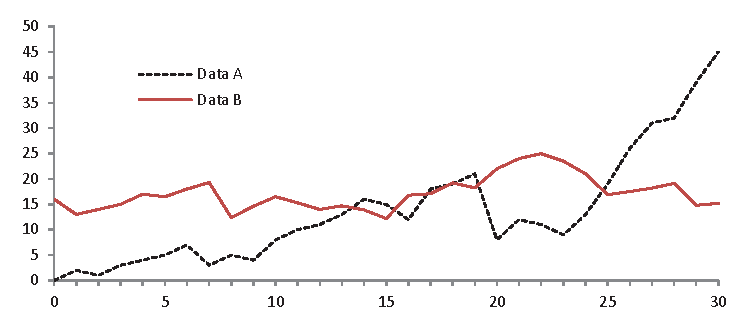
\includegraphics[width=\textwidth]{fig1.eps}
\caption{A figure caption is always placed below the illustration.
Please note that short captions are centered, while long ones are
justified by the macro package automatically.} \label{fig1}
\end{figure}

\begin{theorem}
This is a sample theorem. The run-in heading is set in bold, while
the following text appears in italics. Definitions, lemmas,
propositions, and corollaries are styled the same way.
\end{theorem}
%
% the environments 'definition', 'lemma', 'proposition', 'corollary',
% 'remark', and 'example' are defined in the LLNCS documentclass as well.
%
\begin{proof}
Proofs, examples, and remarks have the initial word in italics,
while the following text appears in normal font.
\end{proof}

\section{Conclusion}


%
% ---- Bibliography ----
%
% BibTeX users should specify bibliography style 'splncs04'.
% References will then be sorted and formatted in the correct style.
%
% \bibliographystyle{splncs04}
% \bibliography{mybibliography}
%
\begin{thebibliography}{8}
\bibitem{ref_article1}
Author, F.: Article title. Journal \textbf{2}(5), 99--110 (2016)

\bibitem{ref_lncs1}
Author, F., Author, S.: Title of a proceedings paper. In: Editor,
F., Editor, S. (eds.) CONFERENCE 2016, LNCS, vol. 9999, pp. 1--13.
Springer, Heidelberg (2016). \doi{10.10007/1234567890}

\bibitem{ref_book1}
Author, F., Author, S., Author, T.: Book title. 2nd edn. Publisher,
Location (1999)

\bibitem{ref_proc1}
Author, A.-B.: Contribution title. In: 9th International Proceedings
on Proceedings, pp. 1--2. Publisher, Location (2010)

\bibitem{ref_url1}
LNCS Homepage, \url{http://www.springer.com/lncs}. Last accessed 4
Oct 2017
\end{thebibliography}
\end{document}
